\section{node2vec}
Algoritmus pro převedení grafu do vektoru nižší dimenze tak aby se s ním dalo dobře pracovat pomocí neuronových sítí.\\
V principu je to ukládání jednotlivých uzlů do vkládacího prostoru o \(d\) dimenzí tak aby "podobné" uzly byly v prostoru blízko sebe.\\

\subsection{Princip}
Algoritmus je založen na algoritmu word2vec užívaném v NLP. Tento algoritmus je využívám pro buď hledání vhodného slova dle kontextu, tedy máme okolní slova a 
jaké bude to chybějící, tomuto se říká CBOW(Continuous Bag Of Words) nebo hledání kontextu podle daného slova, tedy máme slovo a chceme najít slova, která se 
kolem něj často vyskytují, tomuto se říká Skip-Gram.\\
Pro nás je podstatný Skip-Gram, jehož výsledkem jsou slova zakódovaná do vkládacího prostoru, kde jsou slova často se vyskutující spolu blízko u sebe. Ve
skip-gram máme jako vstup hot-one encoded vector, což znamená že slovo kterého chceme znát kontext je nastaveno na 1 a ostatní na 0. Výstupem pak je vektor 
pravděpodobností výskytu ostatních slov kolem našeho žádaného.\\
Místo ve vkládacím prostoru se počítá pomocí natrénované neuronové sítě, kde pomocí vah se určují číselné příznaky slova a podle toho se určuje jeho pozice
ve vkládacím prostoru. Dimenze vkládacích prostorů jsou v praxi většinou mezi 100 a 1000. Tudíž mají 1000 různých příznaků.\\

\begin{figure}[ht]
    \centering
    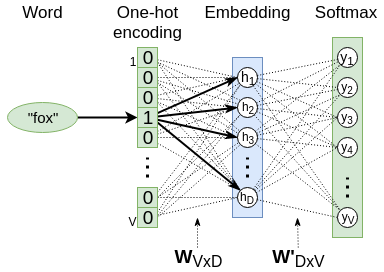
\includegraphics[scale=0.7]{images/skip-gram.png}
\end{figure}

Pro převedení ke zjednušování grafu pak využíváme procházení grafem pro tvorbu těchto "vět". Místo slov však jsou používány samotné ID jednotlivých uzlů. A tím
pádem zjišťujeme kontext uzlů místo kontextu slov ve větě. 

\subsection{Random walk}
Při tomto procházení grafem se postupně od začátečního uzlu náhodně vybere soused a tímto náhodným výběrem se pokračuje dál dokud přejdeme definovaný počet kroků.
Po získání této náhodné cesty se provedem vkládání do prostoru. Poté se zjistí pravděpodobnost navštívení uzlu na cestě z počátečního uzlu \(P(v|u)\) a úhel mezi
jednotlivými vektory ve vkládacím prostoru, toto se provádí vektorovým součinem. Tato pravděpodobnost a úhel by měly být vzájemně proporcionální aby vkládání bylo
správné.
\subsubsection{Optimalizace vkládání}
Optimalizace se provádí tak, že provedeme mnoho krátkých random walks z jednoho uzlu a jejich výsledky vkládáme do multimnožiny \(N_R(u)\). Toto provedeme pro
každý uzel v grafu, takže máme kolekci multimnožin jejichž počet je stejný jako počet uzlů grafu.\\
Následně musíme tyto vkládání optimalizovat. Rovnice kterou se provádí optimalizace je následující:\\
\begin{gather*}
    \mathcal{L} = \sum_{u \in V} \sum_{v \in N_R(u)} -log(P(v|\mathbf{z}_u))
\end{gather*}
Kde \(V\) je množina uzlů v grafu, \(P(v|\mathbf{z}_u)\) je pravděpodobnost výskytu uzlu v na cestě. Tuto pravděpodobnost můžeme pomocí softmaxu parametrizovat:\\
\begin{gather*}
    P(v|\mathbf{z}_u) = \frac{e^{\mathbf{z}_u^T \mathbf{z_v}}}{\sum_{n \in V}e^{\mathbf{z}_u^T \mathbf{z_n}}}
\end{gather*}
Poté tedy získáme:\\
\begin{gather*}
    \mathcal{L} = \sum_{u \in V} \sum_{v \in N_R(u)} -log(\frac{e^{\mathbf{z}_u^T \mathbf{z_v}}}{\sum_{n \in V}e^{\mathbf{z}_u^T \mathbf{z_n}}})
\end{gather*}
Pomocí této rovnice optimalizujeme vkládání tak aby si podobné uzly byly co nejblíže pomocí minimalizace proměnné \(\mathcal{L}\). 

\subsection{Biased walks}
Biased walks se od Random walks liší tím, že nejsou čistě náhodné, ale pomocí parametrů jsme schopni si určit jak by se mělo procházení chovat.\\
\begin{gather*}
    \alpha(t,x)
    \begin{cases}
        \frac{1}{p}; d_{tx} = 0\\
        1; d_{tx} = 1\\
        \frac{1}{q}; d_{tx} = 2\\
    \end{cases}
\end{gather*}
Kde parametry p a q si určujeme a na základě toho se bude walk chovat. Pro procházení okolí uzlu se používají 2 základní strategie, BFS a DFS.\\
\begin{figure}[ht]
    \centering
    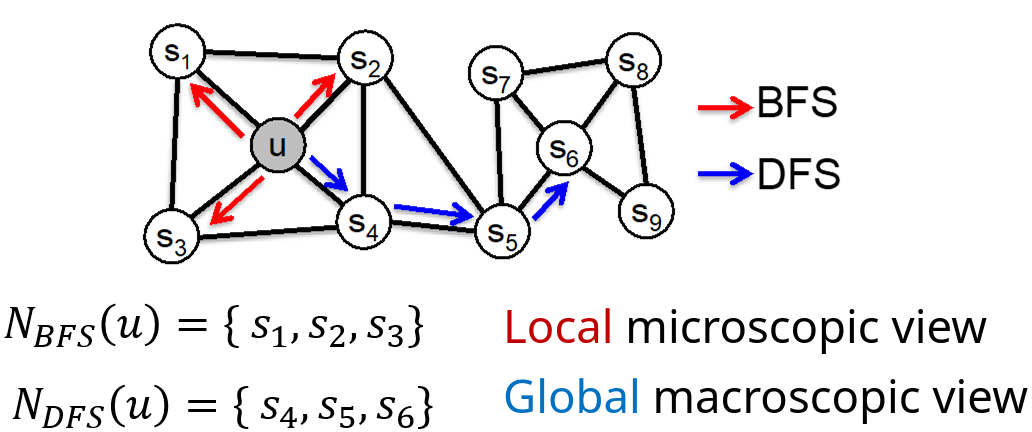
\includegraphics[scale = 0.3]{images/BiasWalk.png}
\end{figure}
\newline
Podle toho jak nastavíme p a q se bude procházení chovat jako DFS nebo BFS. DFS je pro malé hodnoty q a BFS pro malé hodnoty P.\\
\begin{figure}[ht]
    \centering
    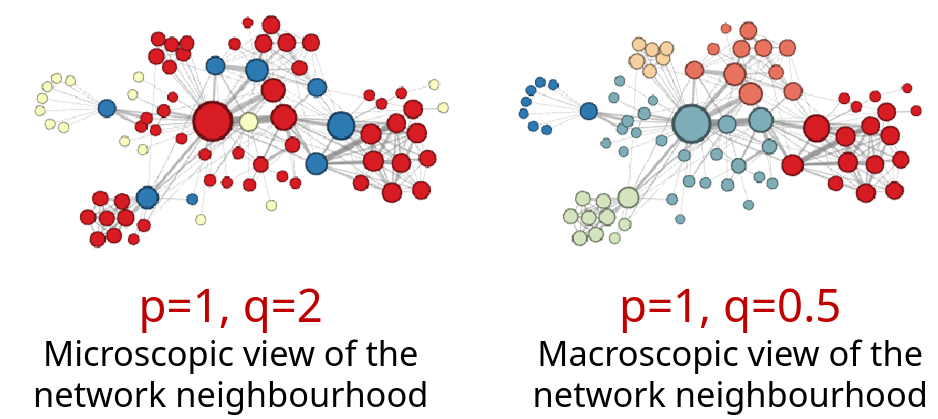
\includegraphics[scale = 0.4]{images/BFSvsDFS.png}
    \caption{Vlevo BFS a vpravo DFS}
\end{figure}